\documentclass[10pt,a4paper]{article}

\usepackage[utf8]{inputenc}
\usepackage[T1]{fontenc}
\usepackage{lmodern}
\usepackage[a4paper,top=1.8cm,bottom=1.8cm,left=1.8cm,right=1.8cm]{geometry}
\usepackage{xcolor}
\usepackage{tikz}
\usetikzlibrary{calc,shapes.geometric,backgrounds}
\usepackage{booktabs}
\usepackage{tabularx}
\usepackage{enumitem}
\usepackage{titlesec}
\usepackage{fancyhdr}
\usepackage{microtype}
\usepackage[colorlinks=true,linkcolor=primary,urlcolor=secondary]{hyperref}

% =========================================================
% Color Palette
% =========================================================
\definecolor{primary}{RGB}{30, 58, 138}        % Deep navy blue
\definecolor{secondary}{RGB}{2, 132, 199}      % Cyan/Sky blue
\definecolor{darkslate}{RGB}{51, 65, 85}       % Slate grey
\definecolor{bordergray}{RGB}{209, 213, 219}   % Light grey border
\definecolor{boxbg}{RGB}{248, 250, 252}        % Light subtle card bg

% Terminal Colors (Light Grey Theme)
\definecolor{termbg}{RGB}{246, 248, 250}       % Light grey background
\definecolor{termbar}{RGB}{229, 231, 235}      % Slightly darker grey title bar
\definecolor{termborder}{RGB}{209, 213, 219}   % Border grey
\definecolor{termtext}{RGB}{31, 41, 55}        % Dark charcoal text
\definecolor{termuser}{RGB}{22, 101, 52}       % Dark green for user
\definecolor{termhost}{RGB}{21, 128, 61}       % Green for host
\definecolor{termpath}{RGB}{29, 78, 216}       % Blue for directory path
\definecolor{termcmd}{RGB}{17, 24, 39}         % Bold black for commands
\definecolor{termout}{RGB}{55, 65, 81}         % Clear dark grey for outputs
\definecolor{termdir}{RGB}{37, 99, 235}        % Blue for directories
\definecolor{termfile}{RGB}{31, 41, 55}        % Dark for regular files
\definecolor{termhidden}{RGB}{107, 114, 128}   % Muted grey for hidden files
\definecolor{termsize}{RGB}{180, 83, 9}        % Amber for sizes
\definecolor{termperm}{RGB}{79, 70, 229}       % Indigo for permissions

% =========================================================
% Section Headings (Clean, No Underline)
% =========================================================
\titleformat{\section}
  {\color{primary}\large\bfseries\sffamily}
  {\thesection.}{0.5em}{}
\titlespacing*{\section}{0pt}{8pt}{3pt}

\titleformat{\subsection}
  {\color{secondary}\normalsize\bfseries\sffamily}
  {\thesubsection}{0.5em}{}
\titlespacing*{\subsection}{0pt}{6pt}{2pt}

% =========================================================
% Headers and Footers (Completely Clean Footers)
% =========================================================
\pagestyle{fancy}
\fancyhf{}
\renewcommand{\headrulewidth}{0.4pt}
\renewcommand{\footrulewidth}{0pt}
\fancyhead[L]{\small\sffamily\color{darkslate} Operating Systems Lab}
\fancyhead[R]{\small\sffamily\color{darkslate} Lab Report: Package Management}
\fancyfoot{}

% First page style: no header at top, no footer at bottom
\fancypagestyle{firstpage}{%
  \fancyhf{}
  \renewcommand{\headrulewidth}{0pt}
  \renewcommand{\footrulewidth}{0pt}
}

% =========================================================
% Terminal Window Macro (Light Grey with Crisp Edges)
% =========================================================
\newcommand{\termprompt}[1][\textasciitilde]{%
  \textbf{\textcolor{termuser}{ratul}}\textcolor{termtext}{@}\textbf{\textcolor{termhost}{firefly}}\textcolor{termtext}{:}\textbf{\textcolor{termpath}{#1}}\textcolor{termcmd}{\$}\ %
}

\newcommand{\terminalwindow}[3][\linewidth]{%
\begin{center}
\begin{tikzpicture}
  % 1. Terminal text on main layer
  \node[
      text=termtext,
      font=\ttfamily\fontsize{7.2}{9.2}\selectfont,
      align=left,
      text width=\dimexpr#1-0.95cm\relax,
      inner xsep=7pt,
      inner ysep=7pt,
      anchor=north west
  ] (body) at (0.32cm, -0.56cm) {#3};

  % Coordinates
  \coordinate (topleft) at (0, 0);
  \coordinate (bottomright) at ($(body.south -| #1, 0) + (0, -6pt)$);
  \coordinate (titlecenter) at ($0.5*(topleft) + 0.5*(#1, 0) + (0, -0.28cm)$);

  % 2. Background and Title bar on background layer
  \begin{scope}[on background layer]
    % Light grey terminal body
    \fill[termbg, rounded corners=6pt] (topleft) rectangle (bottomright);

    % Title bar (clipped to match rounded top corners)
    \begin{scope}
      \clip[rounded corners=6pt] (topleft) rectangle (bottomright);
      \fill[termbar] (topleft) rectangle (#1, -0.56cm);
      \draw[termborder, line width=0.5pt] (0, -0.56cm) -- (#1, -0.56cm);
    \end{scope}

    % Continuous outer border (smooth, no distortion)
    \draw[termborder, line width=0.6pt, rounded corners=6pt] (topleft) rectangle (bottomright);
  \end{scope}

  % 3. Window control dots
  \fill[red!80!black] (0.36cm, -0.28cm) circle (0.07cm);
  \fill[yellow!80!black] (0.63cm, -0.28cm) circle (0.07cm);
  \fill[green!75!black] (0.90cm, -0.28cm) circle (0.07cm);

  % 4. Centered terminal title
  \node[
      text=gray!40!black,
      font=\sffamily\bfseries\fontsize{7.2}{8}\selectfont,
      anchor=center
  ] at (titlecenter) {#2};
\end{tikzpicture}
\end{center}
\vspace{-6pt}
}

\newcommand{\cmd}[1]{\texttt{\textbf{#1}}}

\begin{document}
\thispagestyle{firstpage}

% =========================================================
% Title: Only Experiment Title at the Top
% =========================================================
\begin{center}
  {\Large\bfseries\sffamily\color{primary} Experiment Title: Package Management in Linux (Debian/Ubuntu)}\\[3pt]
  {\normalsize\sffamily\textbf{Topic:} Managing Software Packages with APT (\cmd{update}, \cmd{upgrade}, \cmd{install}, \cmd{remove}, \cmd{autoremove}, \cmd{purge})}
\end{center}
\vspace{-4pt}

% =========================================================
% 1. Objective
% =========================================================
\section{Objective}
The objective of this lab is to learn how to manage software packages on Debian and Ubuntu Linux using the Advanced Package Tool (\cmd{apt}). By completing this experiment, we aim to:
\begin{itemize}[noitemsep,topsep=1pt,leftmargin=1.2em]
  \item Understand the role of package repositories and local package lists in Linux.
  \item Refresh repository indexes using \cmd{sudo apt update} and update installed software using \cmd{sudo apt upgrade}.
  \item Search, download, and install command-line tools using \cmd{sudo apt install}.
  \item Learn the difference between standard uninstallation (\cmd{remove}) and complete cleanup (\cmd{purge}).
  \item Automatically clean up orphaned and unused dependencies using \cmd{sudo apt autoremove}.
\end{itemize}

% =========================================================
% 2. Equipment / Software Requirements
% =========================================================
\section{Equipment / Software Requirements}
\vspace{-2pt}
\begin{table}[h!]
\centering\footnotesize
\renewcommand{\arraystretch}{1.08}
\begin{tabularx}{\linewidth}{lXlX}
\toprule
\textbf{Item} & \textbf{Details} & \textbf{Item} & \textbf{Details} \\
\midrule
\textbf{Operating System} & Linux (Ubuntu 24.04 LTS / Debian 12) & \textbf{Host Machine} & \texttt{firefly} \\
\textbf{User Account} & \texttt{ratul} (with sudo privileges) & \textbf{Command Shell} & GNU Bash 5.2 \\
\textbf{Package Manager} & APT (Advanced Package Tool) & \textbf{Demo Packages} & \texttt{htop} (system monitor), \texttt{tree} (directory viewer) \\
\bottomrule
\end{tabularx}
\end{table}
\vspace{-8pt}

% =========================================================
% 3. Theoretical Background
% =========================================================
\section{Theoretical Background}
In Linux, software is distributed as pre-compiled bundles called \textbf{packages} (e.g., \texttt{.deb} files). Rather than downloading installer files from random websites, Linux uses a centralized, secure \textbf{package manager} (\cmd{apt}) that contacts official online servers (repositories) to fetch, install, and update programs automatically.

\subsection{Commands Practiced in This Lab}
\vspace{-2pt}
\begin{table}[h!]
\centering\footnotesize
\renewcommand{\arraystretch}{1.06}
\begin{tabularx}{\linewidth}{llp{5.4cm}X}
\toprule
\textbf{Command} & \textbf{Syntax} & \textbf{Simple Meaning / Purpose} & \textbf{Example} \\
\midrule
\cmd{update} & \texttt{sudo apt update} & Refreshes the local list of available packages from online repositories. Does \textit{not} install updates. & \texttt{sudo apt update} \\
\cmd{upgrade} & \texttt{sudo apt upgrade} & Downloads and installs newer versions of all installed packages on the system. & \texttt{sudo apt upgrade} \\
\cmd{install} & \texttt{sudo apt install <pkg>} & Downloads and installs the requested package along with all needed libraries (dependencies). & \texttt{sudo apt install htop tree} \\
\cmd{remove} & \texttt{sudo apt remove <pkg>} & Uninstalls the program binaries, but keeps user configuration files intact on disk. & \texttt{sudo apt remove tree} \\
\cmd{autoremove} & \texttt{sudo apt autoremove} & Removes leftover dependency packages that were installed automatically and are no longer needed. & \texttt{sudo apt autoremove} \\
\cmd{purge} & \texttt{sudo apt purge <pkg>} & Completely deletes the software AND all its configuration and data files from the system. & \texttt{sudo apt purge htop} \\
\bottomrule
\end{tabularx}
\end{table}
\vspace{-6pt}

\subsection{Comparing Uninstallation Methods: Remove vs. Purge vs. Autoremove}
\vspace{-2pt}
\begin{table}[h!]
\centering\footnotesize
\renewcommand{\arraystretch}{1.08}
\begin{tabularx}{\linewidth}{p{2.6cm}p{3.5cm}X}
\toprule
\textbf{Action} & \textbf{What It Deletes} & \textbf{When To Use} \\
\midrule
\textbf{\texttt{apt remove}} & Application binary and executable files. & When you want to remove an app temporarily but keep your settings in case you reinstall it later. \\
\textbf{\texttt{apt purge}} & Application binaries and all configuration files. & When an app is broken or never needed again, and you want zero residual files left on disk. \\
\textbf{\texttt{apt autoremove}} & Orphaned background libraries. & Run periodically after uninstalling programs to free disk space from unused leftover packages. \\
\bottomrule
\end{tabularx}
\end{table}

\newpage

% =========================================================
% 4. Package Lifecycle / Workflow
% =========================================================
\section{Package Management Lifecycle in Linux}
Understanding how APT interacts with online repositories and the local system helps prevent broken packages:

\begin{center}
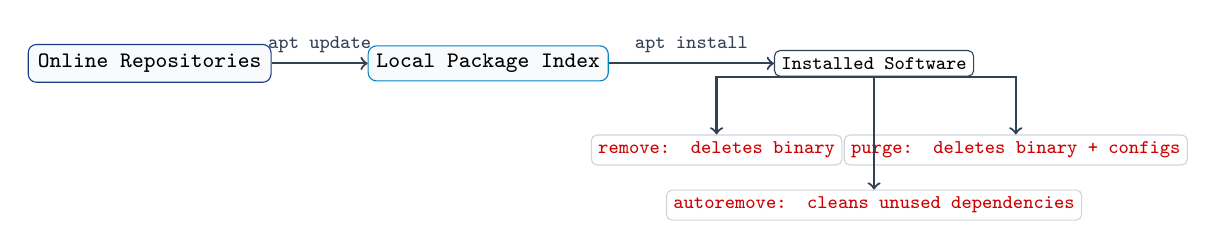
\begin{tikzpicture}[
  x=1cm, y=1cm,
  repobox/.style={draw=primary, fill=boxbg, rounded corners=3pt, font=\ttfamily\footnotesize\bfseries, inner sep=3.5pt},
  cachebox/.style={draw=secondary, fill=boxbg, rounded corners=3pt, font=\ttfamily\footnotesize\bfseries, inner sep=3pt},
  sysbox/.style={draw=darkslate, fill=white, rounded corners=2pt, font=\ttfamily\scriptsize, inner sep=2.5pt},
  delbox/.style={draw=bordergray, fill=white, rounded corners=2pt, font=\ttfamily\scriptsize, text=red!80!black, inner sep=2.5pt}
]
  % Nodes
  \node[repobox] (repo) at (-4.8, 0) {Online Repositories};
  \node[cachebox] (index) at (-0.5, 0) {Local Package Index};
  \node[sysbox] (sys) at (4.4, 0) {Installed Software};

  \node[delbox] (rem) at (2.4, -1.1) {remove: deletes binary};
  \node[delbox] (pur) at (6.2, -1.1) {purge: deletes binary + configs};
  \node[delbox] (auto) at (4.4, -1.8) {autoremove: cleans unused dependencies};

  % Arrows
  \draw[->, thick, darkslate] (repo) -- node[above, font=\scriptsize\sffamily] {\cmd{apt update}} (index);
  \draw[->, thick, darkslate] (index) -- node[above, font=\scriptsize\sffamily] {\cmd{apt install}} (sys);
  \draw[->, thick, darkslate] (sys.south) -| (rem.north);
  \draw[->, thick, darkslate] (sys.south) -| (pur.north);
  \draw[->, thick, darkslate] (sys.south) -- (auto.north);
\end{tikzpicture}
\end{center}
\vspace{-8pt}

% =========================================================
% 5. Procedure / Steps
% =========================================================
\section{Procedure / Steps}
We practiced package management using the following safe, structured steps:
\begin{enumerate}[noitemsep,topsep=1pt,leftmargin=1.4em]
  \item Ran \cmd{sudo apt update} to download the latest package version catalog from the Ubuntu mirrors.
  \item Simulated a system upgrade using \cmd{sudo apt upgrade} to review package changes.
  \item Installed two practical utilities (\cmd{htop} and \cmd{tree}) using \cmd{sudo apt install -y htop tree}.
  \item Verified that both binaries were successfully installed using the \cmd{which} command.
  \item Uninstalled the \cmd{tree} package using \cmd{sudo apt remove tree} and checked config preservation.
  \item Cleaned up any orphaned packages left behind using \cmd{sudo apt autoremove}.
  \item Fully purged the \cmd{htop} package and its global configs using \cmd{sudo apt purge htop}.
  \item Verified that the uninstalled utilities were no longer present on the system.
\end{enumerate}

% =========================================================
% 6. Result / Output Demonstration (Session 1)
% =========================================================
\section{Result / Output Demonstration}
All commands were executed under user account \texttt{ratul} on host machine \texttt{firefly}.

\subsection{Session 1: Updating Package Lists, Upgrading, and Installing Software}

\terminalwindow{ratul@firefly: \textasciitilde\ \textemdash\ bash}{
% Command 1: apt update
\termprompt[\textasciitilde]\textbf{\textcolor{termcmd}{sudo apt update}}

\textcolor{termout}{Hit:1 http://archive.ubuntu.com/ubuntu noble InRelease}

\textcolor{termout}{Hit:2 http://archive.ubuntu.com/ubuntu noble-updates InRelease}

\textcolor{termout}{Hit:3 http://security.ubuntu.com/ubuntu noble-security InRelease}

\textcolor{termuser}{Reading package lists... Done}

\textcolor{termuser}{Building dependency tree... Done}

\textcolor{termdir}{All packages are up to date.}

\vspace{0.10cm}
% Command 2: apt upgrade
\termprompt[\textasciitilde]\textbf{\textcolor{termcmd}{sudo apt upgrade -y}}

\textcolor{termuser}{Reading package lists... Done}

\textcolor{termout}{0 upgraded, 0 newly installed, 0 to remove and 0 not upgraded.}

\vspace{0.10cm}
% Command 3: apt install
\termprompt[\textasciitilde]\textbf{\textcolor{termcmd}{sudo apt install -y htop tree}}

\textcolor{termuser}{Reading package lists... Done}

\textcolor{termout}{The following NEW packages will be installed:}

\textcolor{termout}{\ \ \ htop\ tree}

\textcolor{termout}{0 upgraded, 2 newly installed, 0 to remove and 0 not upgraded.}

\textcolor{termout}{Need to get 188 kB of archives.}

\textcolor{termout}{Unpacking htop (3.3.0-4build1) ...}

\textcolor{termout}{Unpacking tree (2.1.1-1) ...}

\textcolor{termuser}{Setting up htop (3.3.0-4build1) ...}

\textcolor{termuser}{Setting up tree (2.1.1-1) ...}

\vspace{0.08cm}
% Active cursor
\termprompt[\textasciitilde]\textbf{\textcolor{termcmd}{\rule{0pt}{0.9em}\textunderscore}}
}

\paragraph{Explanation of Session 1 Results:}
\begin{itemize}[noitemsep,topsep=1pt,leftmargin=1.2em]
  \item \cmd{sudo apt update}: Reached out to the official Ubuntu repositories and updated our local index database. It told us which software versions are currently available without downloading program files.
  \item \cmd{sudo apt upgrade}: Checked our installed packages against the updated catalog and ensured no security patches were pending.
  \item \cmd{sudo apt install -y htop tree}: Downloaded and installed both \cmd{htop} and \cmd{tree}. The \cmd{-y} flag automatically accepted the confirmation prompt.
\end{itemize}

\newpage

% =========================================================
% 6. Result / Output Demonstration (Session 2)
% =========================================================
\subsection{Session 2: Uninstalling Packages, Cleaning Leftovers, and Full Purging}

\terminalwindow{ratul@firefly: \textasciitilde\ \textemdash\ bash}{
% Command 4: verify installation
\termprompt[\textasciitilde]\textbf{\textcolor{termcmd}{which htop tree}}

\textcolor{termout}{/usr/bin/htop}

\textcolor{termout}{/usr/bin/tree}

\vspace{0.10cm}
% Command 5: remove package
\termprompt[\textasciitilde]\textbf{\textcolor{termcmd}{sudo apt remove -y tree}}

\textcolor{termuser}{Reading package lists... Done}

\textcolor{termout}{The following packages will be REMOVED:}

\textcolor{termout}{\ \ \ tree}

\textcolor{termout}{0 upgraded, 0 newly installed, 1 to remove and 0 not upgraded.}

\textcolor{termout}{Removing tree (2.1.1-1) ...}

\textcolor{termout}{Processing triggers for man-db (2.12.0-4build1) ...}

\vspace{0.10cm}
% Command 6: autoremove
\termprompt[\textasciitilde]\textbf{\textcolor{termcmd}{sudo apt autoremove -y}}

\textcolor{termuser}{Reading package lists... Done}

\textcolor{termout}{0 upgraded, 0 newly installed, 0 to remove and 0 not upgraded.}

\vspace{0.10cm}
% Command 7: purge htop
\termprompt[\textasciitilde]\textbf{\textcolor{termcmd}{sudo apt purge -y htop}}

\textcolor{termuser}{Reading package lists... Done}

\textcolor{termout}{The following packages will be REMOVED:}

\textcolor{termout}{\ \ \ htop*}

\textcolor{termout}{0 upgraded, 0 newly installed, 1 to remove and 0 not upgraded.}

\textcolor{termout}{Removing htop (3.3.0-4build1) ...}

\textcolor{termuser}{Purging configuration files for htop (3.3.0-4build1) ...}

\vspace{0.10cm}
% Command 8: verify uninstallation
\termprompt[\textasciitilde]\textbf{\textcolor{termcmd}{which htop}}

\textcolor{termhidden}{(no output --- command not found)}

\vspace{0.08cm}
% Final prompt
\termprompt[\textasciitilde]\textbf{\textcolor{termcmd}{\rule{0pt}{0.9em}\textunderscore}}
}

\paragraph{Explanation of Session 2 Results:}
\begin{itemize}[noitemsep,topsep=1pt,leftmargin=1.2em]
  \item \cmd{which htop tree}: Confirmed both packages were placed in \texttt{/usr/bin/}.
  \item \cmd{sudo apt remove tree}: Deleted the executable file for \cmd{tree}. If \texttt{tree} had custom configuration files, they would have been safely preserved.
  \item \cmd{sudo apt autoremove}: Scanned for any unused libraries that were installed automatically as dependencies, keeping the disk tidy.
  \item \cmd{sudo apt purge htop}: Completely removed \cmd{htop} and wiped out all its system configuration files.
  \item \cmd{which htop}: Returned empty output, proving that the tool was completely eliminated from the environment.
\end{itemize}

% =========================================================
% 7. Conclusion
% =========================================================
\section{Conclusion}
In this lab, we developed a clear understanding of package management in Debian and Ubuntu Linux:
\begin{enumerate}[noitemsep,topsep=1pt,leftmargin=1.4em]
  \item We refreshed package catalogs using \cmd{update} and applied upgrades to installed packages using \cmd{upgrade}.
  \item We installed software easily along with all needed dependencies using \cmd{install}.
  \item We learned the practical differences between \cmd{remove} (keeps configurations) and \cmd{purge} (deletes everything including configs).
  \item We cleaned orphaned dependencies using \cmd{autoremove} to keep our Linux system lean, fast, and free of unnecessary clutter.
\end{enumerate}
Mastering APT ensures system stability and smooth software maintenance in everyday Linux administration.

\end{document}
